\documentclass[12pt]{report}
\usepackage[left=2.5cm, right=2.5cm, top=1.5cm, bottom=2cm]{geometry}
\usepackage[utf8]{vietnam}
\usepackage{graphicx}
\title{\textbf{Báo cáo môn Hệ điều hành} \\ \textbf{Deadlock}}
\author{Nguyễn Duy Đạt 20215343}
\usepackage{lmodern}
\usepackage{setspace}
\renewcommand{\baselinestretch}{1.2}
\date{}
\begin{document}

\maketitle
\begin{abstract}
	\textbf{Deadlock} (\textbf{Bế tắc}) là một khái niệm quan trọng trong Hệ điều hành. \vspace{2mm}
	
	Trong bối cảnh ngày càng tăng của các hệ thống đa nhiệm và đa người dùng, việc hiểu và xử lý deadlock là một phần cực kỳ thiết yếu trong việc thiết kế và quản lý hệ thống. Deadlock có thể ảnh hưởng đáng kể đến hiệu suất và độ ổn định của hệ thống, và điều này đặc biệt đúng đối với các hệ thống quy mô lớn.
	\vspace{2mm} 
	
	Trong bài viết này, chúng ta sẽ tìm hiểu khái niệm deadlock, các điều kiện cần để xảy ra deadlock và các phương pháp, giải thuật để xử lý deadlock, bao gồm các chiến lược phòng ngừa, phòng tránh, nhận biết và khắc phục.
	\vspace{2mm}
	
	Bên cạnh đó, chúng ta cũng sẽ khám phá các ví dụ và ứng dụng thực tế của xử lý bế tắc, cụ thể hơn là trong hệ điều hành Windows.
\end{abstract}
\section*{I. Khái niệm}
\textbf{Deadlock} (\textbf{Bế tắc}) là tình trạng 
\begin{itemize}
	\item Hai hay nhiều tiến trình bị mắc kẹt và không thể tiếp tục thực hiện vì chúng đang chờ đợi tài nguyên dùng chung (tài nguyên găng) mà tiến trình khác đang chiếm giữ.
	\item Nếu không có sự tác động gì từ bên ngoài, thì các tiến trình sẽ phải chờ đợi vô hạn.
\end{itemize}
\section*{II. Điều kiện xảy ra bế tắc}
Các điều kiện xảy ra bế tắc thường được gọi là \textbf{bốn điều kiện cần} và bao gồm:

\begin{itemize}
	\item \textbf{Tài nguyên găng}: Mỗi tiến trình yêu cầu sử dụng một tài nguyên không phân chia được và chỉ có thể được giải phóng khi tiến trình khác đang sử dụng nó hoàn thành.
	\item \textbf{Chờ đợi}: Các tiến trình phải xếp hàng chờ đợi tài nguyên, trong khi chờ đợi vẫn chiếm giữ tài nguyên đã được cung cấp trước đó.
	\item \textbf{Trưng dụng tài nguyên găng}: Các tài nguyên chỉ có thể bị giải phóng khi tiến trình đang nắm giữ đã hoàn thành nhiệm vụ.
	\item \textbf{Chờ đợi vòng tròn}: Tồn tại một chuỗi các tiến trình đang chờ đợi tài nguyên mà tiến trình cuối cùng trong chuỗi lại chờ đợi tài nguyên do tiến trình đầu tiên trong chuỗi nắm giữ: ${P_0,P_1,\ldots,P_n,P_0,\ldots}$
\end{itemize}

Hiểu rõ các điều kiện cần này sẽ giúp chúng ta nhận biết và phân tích các tình huống bế tắc trong hệ thống, từ đó đưa ra các giải pháp và phương pháp xử lý hợp lý.

\section*{III. Các phương pháp xử lý bế tắc}
Trong phần này, chúng ta sẽ xem xét các phương pháp khác nhau để xử lý bế tắc trong hệ thống. Các phương pháp này có thể được chia thành ba mục như sau:

\subsection*{1. Phòng ngừa bế tắc}
\subsubsection*{Đặc điểm}
\begin{itemize}
	\item Hạn chế tối đa tình trạng hệ thống rơi vào bế tắc.
	\item Tốn kém, thường áp dụng cho hệ thống dễ xảy ra bế tắc và tổn thất xảy ra lớn.
\end{itemize}
\subsubsection*{Phương pháp}
Tác động vào một trong các điều kiện cần của bế tắc để nó không xảy ra:
\begin{itemize}
	\item Điều kiện tài nguyên găng:
	      \begin{itemize}
	      	\item Giảm mức độ chia sẻ tài nguyên.
	      	\item Không phân phối tài nguyên khi không thật sự cần thiết.
	      	\item Hạn chế số tiến trình có thể yêu cầu tài nguyên.
	      \end{itemize}
	\item Chờ đợi trước khi vào đoạn găng:
	                  
	      Đảm bảo một tiến trình xin tài nguyên khi nó đang không chiếm giữ tài nguyên nào
	      \begin{itemize}
	      	\item Xin toàn bộ tài nguyên ngay từ đầu: có thể vượt quá khả năng của hệ thống.
	      	\item Giải phóng toàn bộ tài nguyên trước khi xin tài nguyên mới: tốc độ chậm.
	      \end{itemize}
	\item Điều kiện trưng dụng tài nguyên : 
	      \begin{itemize}
	      	\item Hạn chế việc tiến trình giữ tài nguyên một cách độc quyền mà không cho phép chia sẻ với các tiến trình khác.
	      	\item Lưu lại trạng thái của tiến trình và giải phóng tài nguyên cho các tiến trình đang cần, sau đó khôi phục lại.
	      	\item Thường được áp dụng cho các tài nguyên mà trạng thái của nó có thể dễ dàng lưu lại và được khôi phục sau đó, chẳng hạn như các thanh ghi CPU và bộ nhớ.
	      \end{itemize}
	\item Chờ đợi vòng tròn : 
	      \begin{itemize}
	      	\item Đặt ra một thứ tự tổng thể của
	      	      tất cả các loại tài nguyên và buộc mỗi tiến trình yêu cầu tài nguyên theo một thứ tự tăng dần.
	      \end{itemize}
\end{itemize}

\subsection*{2. Phòng tránh bế tắc}
\subsubsection*{Đặc điểm}
\begin{itemize}
	\item Kiểm tra các yêu cầu tài nguyên, không chấp nhận cấp phát nếu có thể xảy ra bế tắc.
	\item Thường yêu cầu các thông tin phụ trợ.
	\item Áp dụng cho hệ thống ít xảy ra bế tắc nhưng thiệt hại lớn.
\end{itemize}
\subsubsection*{Phương pháp}
Có hai thuật toán chính để phòng tránh bế tắc, bao gồm:
\begin{itemize}
	\item Dựa vào đồ thị cung cấp tài nguyên:
	      \begin{itemize}
	      	\item Dựa trên cơ chế phân tích đồ thị cung cấp tài nguyên (Resource Allocation Graph - RAG) để xác định khả năng xảy ra deadlock. Đồ thị này sẽ mô tả quan hệ giữa các tiến trình và tài nguyên, cho phép phát hiện chu trình chờ đợi và ngăn chặn tình trạng deadlock.
	      	\item Được sử dụng để quản lý việc cấp phát và thu hồi tài nguyên cho các tiến trình, đồng thời đảm bảo rằng không có chu trình chờ đợi trong đồ thị.
	      \end{itemize}
	      \begin{figure}[ht]
	      	\centering
	      	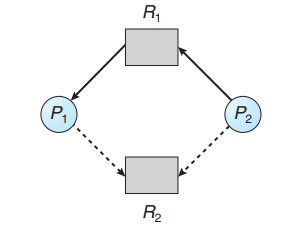
\includegraphics{resources/rag.png}
	      	\caption{Ví dụ về đồ thị cung cấp tài nguyên}
	      	\label{fig:enter-label}
	      \end{figure}
	          
	\item Thuật toán Banker's: 
	      \begin{itemize}
	      	\item Là một thuật toán phòng tránh bế tắc phổ biến. Nó kiểm tra xem có thể cấp phát tài nguyên cho một yêu cầu mới mà không gây ra deadlock hay không bằng cách đánh giá tài nguyên còn lại của hệ thống và tài nguyên yêu cầu của các tiến trình khác.
	      	\item Nếu không gây ra deadlock, thuật toán đảm bảo một thứ tự an toàn cho các tiến trình thực hiện.
	      \end{itemize}
	      \begin{table}[htbp]
	      	\centering
	      	\begin{tabular}{|c|c|c|c|c|}
	      		\hline
	      		Process & Allocation  & Max         & Need        & Available   \\
	      		\hline
	      		$P_1$   & $(0, 1, 0)$ & $(7, 5, 3)$ & $(7, 4, 3)$ & $(3, 3, 2)$ \\
	      		$P_2$   & $(2, 0, 0)$ & $(3, 2, 2)$ & $(1, 2, 2)$ &             \\
	      		$P_3$   & $(3, 0, 2)$ & $(9, 0, 2)$ & $(6, 0, 0)$ &             \\
	      		$P_4$   & $(2, 1, 1)$ & $(2, 2, 2)$ & $(0, 1, 1)$ &             \\
	      		\hline
	      	\end{tabular}
	      	\caption{Bảng mô tả thuật toán Banker's}
	      \end{table}
\end{itemize}

\subsection*{3. Nhận biết và khắc phục}
\subsubsection*{Đặc điểm}
\begin{itemize}
	\item Cho phép bế tắc xảy ra.
	\item Định kì kiểm tra bế tắc có xảy ra hay không, nếu có thì khắc phục.
	\item Áp dụng cho hệ thống ít xảy ra bế tắc và thiệt hại không lớn.
\end{itemize}
\subsubsection*{Phương pháp}
\begin{itemize}
	\item Nhận biết:
	      \begin{itemize}
	      	\item Sử dụng đồ thị cung cấp tài nguyên: Nếu đồ thị có chu trình, hệ thống lúc này đang bế tắc.
	      	\item Giải thuật Banker's: Ngoài việc phòng tránh bế tắc, thuật toán Banker's cũng có thể được sử dụng để nhận biết bế tắc. Bằng cách kiểm tra trạng thái hiện tại của hệ thống và yêu cầu tài nguyên từ các tiến trình, ta có thể phát hiện sự tồn tại của deadlock.
	      \end{itemize}
	\item Khi nào nên sử dụng các thuật toán nhận biết?
	          
	      Nếu bế tắc xảy ra thường xuyên, ta nên dùng các thuật toán \textit{Nhận biết} thường xuyên. Tuy nhiên, việc sử dụng thuật toán cho mỗi yêu cầu tài nguyên sẽ tốn kém về mặt tính toán. Một lựa chọn ít tốn kém hơn là sử dụng thuật toán theo từng khoảng thời gian xác định hoặc theo tiêu chí như tỷ lệ sử dụng CPU.
	\item Khắc phục:
	      \begin{itemize}
	      	\item Kết thúc tiến trình:
	      	      \begin{itemize}
	      	      	\item Hủy bỏ tất cả tiến trình: nhanh chóng nhưng tốn kém.
	      	      	\item Hủy bỏ lần lượt cho đến khi bế tắc không xảy ra: Sau mỗi lần hủy bỏ, phải kiểm tra lại tình trạng bế tắc.
	      	      \end{itemize}
	      	\item Trưng dụng tài nguyên:
	      	      \begin{itemize}
	      	      	\item Rollback: quay lui đến trạng thái an toàn trước đó và bắt đầu lại, yêu cầu lưu lại thông tin tiến trình đang thực hiện.
	      	      	\item Starvation: ghi lại số lần trưng dụng, tránh tiến trình phải chờ đợi quá lâu.
	      	      \end{itemize}
	      \end{itemize}
	      % 
\end{itemize}

\section*{IV. Phát hiện và xử lý bế tắc trong Windows}
Hệ điều hành Windows xử lý deadlock thông qua các cơ chế và chiến lược khác nhau nhằm ngăn chặn, phát hiện và giải quyết các tình huống deadlock. Dưới đây là một số cách mà Windows xử lý deadlock:

\subsection*{1. Sắp xếp khóa}
Windows áp dụng giao thức sắp xếp khóa để đảm bảo việc lấy và giải phóng khóa nhất quán. Bằng cách tuân theo một thứ tự đã định trước, ví dụ như lấy khóa theo thứ tự tăng dần của địa chỉ bộ nhớ, Windows giảm thiểu khả năng xảy ra deadlock.
\subsection*{2. Phát hiện deadlock}
Windows sử dụng các thuật toán và kỹ thuật phát hiện deadlock để xác định các deadlock tiềm năng. Ví dụ, công cụ Driver Verifier trong Windows có thể phát hiện vi phạm thứ tự khóa và deadlock tiềm năng bằng cách xây dựng đồ thị về thứ tự lấy tài nguyên và kiểm tra vòng lặp. Sau khi phát hiện deadlock, các biện pháp thích hợp có thể được thực hiện.
\subsection*{3. Quản lý tài nguyên}
Windows cung cấp các cơ chế để quản lý tài nguyên một cách hiệu quả và giảm thiểu khả năng xảy ra deadlock. Ví dụ, chính sách phân bổ tài nguyên như thuật toán Banker có thể được sử dụng để đảm bảo phân bổ tài nguyên an toàn và tránh deadlock tiềm ẩn.
\subsection*{4. Đặt thời gian chờ}
Windows thường sử dụng thời gian chờ như một biện pháp ngăn chặn deadlock. Nếu một luồng không thể lấy khóa trong một khoảng thời gian nhất định, nó có thể giải phóng các khóa hiện đang nắm giữ và thử lại sau, từ đó ngăn chặn deadlock tiềm ẩn.
\subsection*{5. Giải quyết deadlock}
Windows áp dụng các chiến lược khác nhau để giải quyết deadlock. Một phương pháp thông thường là sử dụng kỹ thuật \textbf{tránh deadlock (deadlock avoidance)}, trong đó hệ thống phân tích đồ thị phân bố tài nguyên để xác định xem một yêu cầu tài nguyên cụ thể có dẫn đến deadlock hay không. Nếu dự đoán có deadlock, hệ thống có thể chọn từ chối yêu cầu tài nguyên để tránh tình huống deadlock.
\subsection*{6. Công cụ giám sát và gỡ lỗi hệ thống}
Windows cung cấp các công cụ và tiện ích để giám sát, chẩn đoán và gỡ lỗi deadlock bao gồm Task Manager, Resource Monitor, Event Viewer và các công cụ gỡ lỗi như WinDbg,\ldots Những công cụ này giúp quản trị viên và nhà phát triển xác định và giải quyết các vấn đề liên quan đến deadlock.
\begin{figure}[ht]
	\centering
	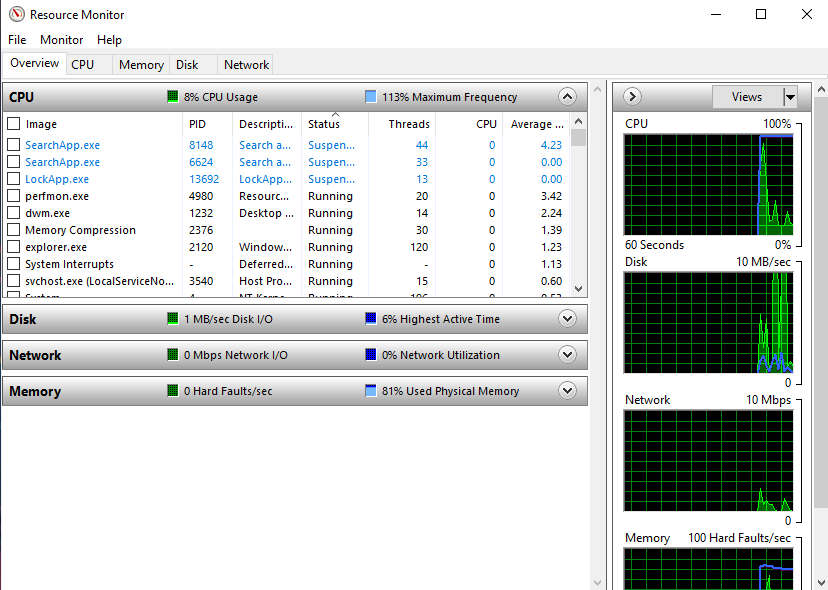
\includegraphics[width=10cm]{resources/resource_monitor.png}
	\caption{Tiện ích Resource Monitor trên Windows}
\end{figure}

\vspace{2mm}
Nhìn chung, Windows kết hợp các chiến lược ngăn chặn, phát hiện và giải quyết để xử lý deadlock một cách hiệu quả, đảm bảo sự ổn định và đáng tin cậy của hệ thống.

\section*{V. Một số ứng dụng thực tế}

Hệ điều hành và các thuật toán xử lý bế tắc có ứng dụng rộng rãi trong các môi trường thực tế để đảm bảo hiệu suất và đáng tin cậy của hệ thống. Dưới đây là một số ứng dụng:

\subsection*{1. Hệ thống máy tính đa nhiệm}
Trong hệ thống máy tính đa nhiệm, nhiều tiến trình chạy đồng thời và chia sẻ các tài nguyên hệ thống. Để đảm bảo không xảy ra bế tắc, hệ điều hành áp dụng các thuật toán phòng ngừa và phòng tránh bế tắc để quản lý việc cấp phát và giải phóng tài nguyên cho các tiến trình.

\subsection*{2. Cơ sở dữ liệu phân tán}
Trong cơ sở dữ liệu phân tán, nhiều hệ thống cơ sở dữ liệu hoạt động song song và truy cập vào các tài nguyên phân tán. Xử lý bế tắc trong môi trường này đòi hỏi việc áp dụng các thuật toán phòng tránh và nhận biết bế tắc để đảm bảo tính nhất quán và sẵn sàng của cơ sở dữ liệu.

\subsection*{3. Hệ thống máy chủ web}
Trong môi trường máy chủ web, nhiều yêu cầu truy cập đồng thời đến các tài nguyên như bộ nhớ, ổ đĩa và mạng. Quản lý tài nguyên và xử lý bế tắc là một phần quan trọng trong việc đảm bảo sự phản hồi nhanh chóng và ổn định của máy chủ web. Các thuật toán và khái niệm liên quan đến bế tắc được áp dụng để tăng cường hiệu suất và độ tin cậy của hệ thống máy chủ web.
\section*{VI. Kết luận}

Trên đây, chúng ta đã tìm hiểu về bế tắc, các điều kiện xảy ra bế tắc và các thuật toán phòng ngừa, phòng tránh và nhận biết bế tắc.\vspace{2mm}

Các phương pháp này đã được áp dụng rộng rãi trong nhiều lĩnh vực thực tế như hệ thống máy tính, mạng, cơ sở dữ liệu và sản xuất công nghiệp. Chúng giúp tối ưu hóa sử dụng tài nguyên và đảm bảo hoạt động ổn định của hệ thống.\vspace{2mm}

Từ kiến thức này, chúng ta có thể xây dựng và duy trì các hệ thống hiệu suất cao và đáng tin cậy. Việc nghiên cứu và phát triển thuật toán mới cũng đóng góp vào việc nâng cao khả năng xử lý bế tắc trong các hệ thống tương lai.
\end{document}